\documentclass[12pt]{article}
%Gumm{\color{blue}i}|065|=)
\usepackage{amsmath, amsfonts, amssymb}
\usepackage[margin=0.5in]{geometry}
\usepackage{xcolor}
\usepackage{graphicx}
\usepackage{amsmath}
\usepackage{hyperref}

\newcommand{\off}[1]{}
\DeclareMathSizes{20}{30}{20}{18}
\usepackage{tikz}


\title{Scratchwork: Sudoku}
\date{}
\begin{document}

\sffamily

\maketitle

\noindent  Let's try to solve Sudoku as an integer progrmaming problem.  There are many acceptable answers.  \\ \\
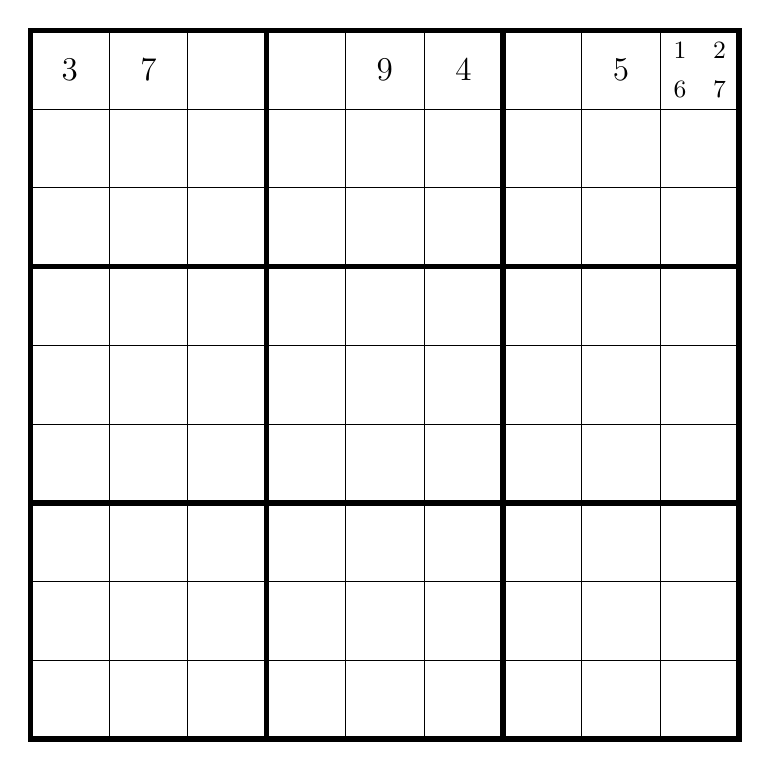
\begin{tikzpicture}
\foreach \a in {0,3,...,9}{
	\foreach \b in {0,3,...,9}{
		\draw[line width=2] (0,0)--(\a,0)--(\a,\b)--(0,\b)--cycle;
	}
}

\foreach \a in {0,1,...,9}{
	\draw (0,\a)--(9,\a);
	\draw (\a,0)--(\a,9);
}

\node at (0+0.5,9-0-0.5) {\large 3};
\node at (1+0.5,9-0-0.5) {\large 7};
\node at (4+0.5,9-0-0.5) {\large 9};
\node at (5+0.5,9-0-0.5) {\large 4};
\node at (7+0.5,9-0-0.5) {\large 5};
\node at (8+0.25,9-0-0.25) {\small 1};
\node at (8+0.75,9-0-0.25) {\small 2};
\node at (8+0.25,9-0-0.75) {\small 6};
\node at (8+0.75,9-0-0.75) {\small 7};

\end{tikzpicture} \\ \\
We can solve this problem \textit{twice}.  Once with Linear Algebra, and again piping that linear algebra into programs like COIN-OR or possibly \texttt{numPy}, with Python or Julia language.  The data structure common to all of these will be \texttt{[integer]} and \texttt{Array}.  We'll solve a system of linea inequality with 100 equations and 800 unknowns, with values in $\{0,1\}$. \\ \\
\textbf{Example} How do we formalize the notion of square, where we know some of the values but not enough of them to put in a number?  \\ \\ 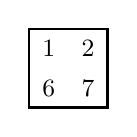
\begin{tikzpicture}[scale=1] 
\draw[line width = 1] (0,0)--(1,0)--(1,1)--(0,1)--cycle;
\node at (0+0.25,1-0-0.25) {\small 1};
\node at (0+0.75,1-0-0.25) {\small 2};
\node at (0+0.25,1-0-0.75) {\small 6};
\node at (0+0.75,1-0-0.75) {\small 7};
\end{tikzpicture} \\ 
\textbf{Example} How do we formalize that moment when because we know the value at one square, we can ignore all the othe rsquares it the row?  \\ 
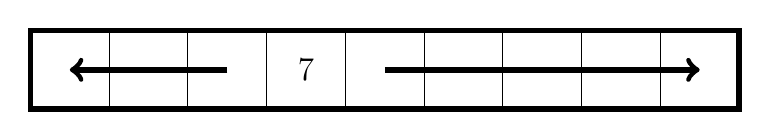
\begin{tikzpicture}[scale=1]
\draw[line width=2] (0,0)--(9,0)--(9,1)--(0,1)--cycle;
\foreach \a in {0,1,...,9}{
	\draw (\a,0)--(\a,1);
}
\node at (3+0.5,1-0.5) {\large 7};
\draw[line width=2, ->] (4.5,0.5)--(8.5,0.5);
\draw[line width=2, ->] (2.5,0.5)--(0.5,0.5);
\end{tikzpicture} \\ 
We could encode this sudoku as a $9 \times 9 \times 9$ array, $x_{ijk}$ with $0 \leq i,j,k < 9$.  If we set $x_{ijk} = 1$ we are saying there is the value $k$ at the square $(i,j)$.  And $x_{ijk}=0$ if the number is not there. Our constraints read:
\begin{itemize}
\item $x_{ijk} \in \{ 0,1\}$
\item each square contains a number $\displaystyle \sum_{k} x_{ijk} = 1$
\item each row contains a number $\displaystyle \sum_{i} x_{ijk} = 1$
\item each column contains a number $\displaystyle \sum_{j} x_{ijk} = 1$
\item each $3 \times 3$ block contains a number $\displaystyle \sum_{(i,j) \in 3 \times 3} x_{ijk}=1$
\end{itemize} 
We now have to tell our computer how to describe the same thing.  \texttt{x[i][j][k]} \\ \\
The integer programming textbook lumps all problems of this kind into the same format $Ax \leq b$ where $A$ is some $m \times n$ matrix representing all linear constraints and $b$ is a $n \times 1$ vector containing all the numbers.  How do we list all of our Sudoku rules as ``constraints" and linear inequalities?

\newpage

\noindent 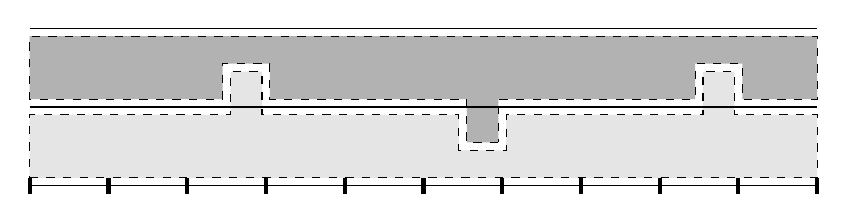
\begin{tikzpicture}

\draw[dashed,fill=black!10!white] (0,0.1)--(10,0.1)--(10,0.9)--(8.95,0.9)--(8.95,1.45)--(8.55,1.45)--(8.55,0.9)--(6.05,0.9)--(6.05,0.45)--(5.45,0.45)--(5.45,0.9)--(2.95,0.9)--(2.95,1.45)--(2.55,1.45)--(2.55,0.9)--(0,0.9)--cycle;

\draw[dashed, fill=black!30!white] (5.95,0.55)--(5.55,0.55)--(5.55,1.1)--(3.05,1.1)--(3.05,1.55)--(2.45,1.55)--(2.45,1.1)--(0,1.1)--(0,1.9)--(10,1.9)--(10,1.1)--(9.05,1.1)--(9.05,1.55)--(8.45,1.55)--(8.45,1.1)--(5.95,1.1)--cycle;

\draw (0,2)--(10,2);

\draw (0,1)--(10,1);

\draw (0,0)--(10,0);

\foreach \a  in {0,...,10}{
	\draw[line width = 1.5] (\a,-0.1)--(\a,0.1);
}

 \end{tikzpicture}

\vfill
\begin{thebibliography}{} 
\item \textbf{Optimization Methods in Business Analytics} \texttt{http://web.mit.edu/15.053/www/}
\item Michele Conforti, G\'{e}rard Cornuejols, Giacomo Zambelli. \textbf{Integer Programming} (GTM \#271) Springer, 2014.
\end{thebibliography}
\end{document}